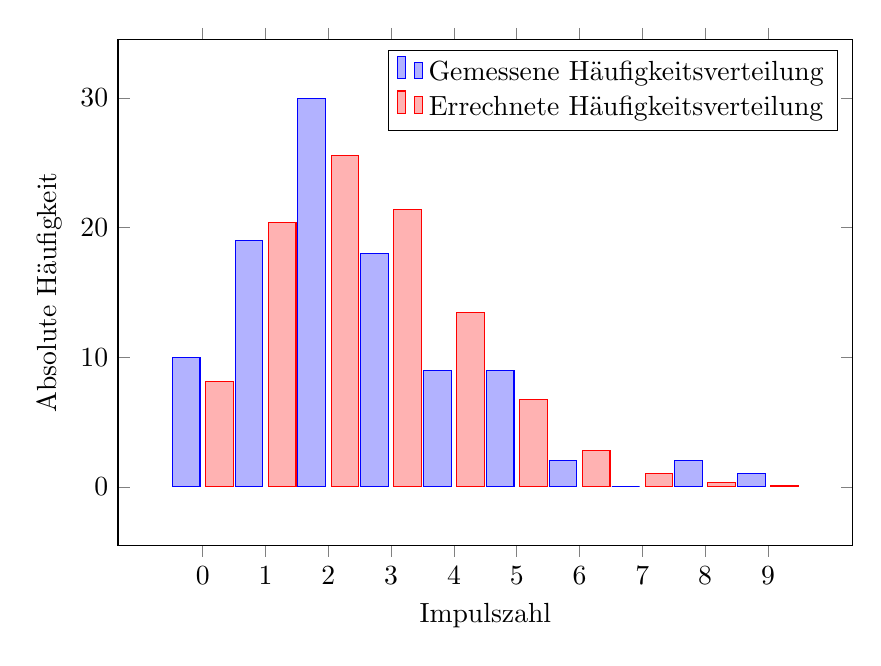
\begin{tikzpicture}[]
\begin{axis} [
width=.9\textwidth,
height = 8cm,
enlargelimits=.15,
ybar,
%bar width = 5pt,
%symbolic x coords={excellent, good, neutral},
%nodes near coords,
xtick = data,
xlabel={Impulszahl},
ylabel={Absolute Häufigkeit},
]
\addplot coordinates {(0, 10)
	(1, 19)
	(2, 30)
	(3, 18)
	(4, 9)
	(5, 9)
	(6, 2)
	(7, 0)
	(8, 2)
	(9, 1)
};
\addlegendentry{Gemessene Häufigkeitsverteilung};
\addplot table[x = x, y=y] {
x y
0	8.1268239241
1	20.3983280495
2	25.5999017021
3	21.4185844241
4	13.4401617261
5	6.7469611865
6	2.822478763
7	1.0120602422
8	0.317533901
9	0.0885566768
};
\addlegendentry{Errechnete Häufigkeitsverteilung};
\end{axis}
\end{tikzpicture}